\section{Vegetation}

Vegetation is core to rural landscapes. The species present along with their associated densities create a relationship between ecotopes and areas on earth on which resources are adequate. To ensure realism in virtual rural worlds, much emphasize must be put on efficiently modelling these underlying ecosystems.\\

This section will review different methods to generate suitable vegetation for virtual worlds. These methods will be split into three main categories: \textit{Explicit instancing, probabilistic instancing} and \textit{ecosystem simulators}.\\
\textit{Explicit instancing} use user input to either directly or indirectly pinpoint exact locations for individual plant instances.\\
\textit{probabilistic instancing} methods use statistical models to generate suitable vegetation.\\ 
\textit{ecosystem simulators} attempt to reproduce plants battling for available resources algorithmically.\\

\subsection{Explicit Instancing} \label{Explicit Instancing}
Explicit instancing methods require input from the user to explicitly outline the location of individual plant instances. \\
Arnaud et al. \cite{Emilien} permit users to insert individual plants manually by simply clicking the appropriate location on the terrain. To overcome the tedious task of manually placing individual plant instances on large terrains, the system is able to analyse existing distributions for reproduction. For example, to generate a large forest, the user is only required to generate a small subsection which can then be used to reproduce it on any scale (figure \ref{Explicit instancing as input examplars}) \\

\begin{figure}[h]
  \centering
	\label{Explicit instancing as input examplars}
	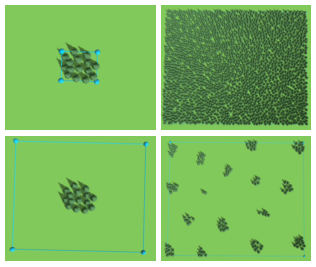
\includegraphics[natwidth=316,natheight=267]{worldbrush_forrest_reproduction.png}
	\caption{Using explicit instancing as input examplars for reproduction \cite{Emilien}}
\end{figure}

Similarly, Deussen et al. \cite{Deussen1998} allow users to use grayscale raster images as input to specify terrain vegetation. The location of individual plants is determined by pixel location whereas plant properties are correlated to pixel intensity.\\

During their work focused on improving the realism of roadside landscapes, C. Andujar et al. ~\cite{Andujar2014} use orthophotos as input to determine the location and properties of individual plants. Unlike ordinary aerial photographs, aerial orthophotos use normalisation techniques to take into account terrain relief and camera tilt to produce the image. The result is an image with uniform scale throughout, which, similarly to a map, can be used to accurately measure distances between points. Here, the orthophotos are analysed to determine the center point of individual plants.\\

\begin{figure}[!htb]
  \centering
	\label{Reconstructed roadside vegetation using orthophotos}
	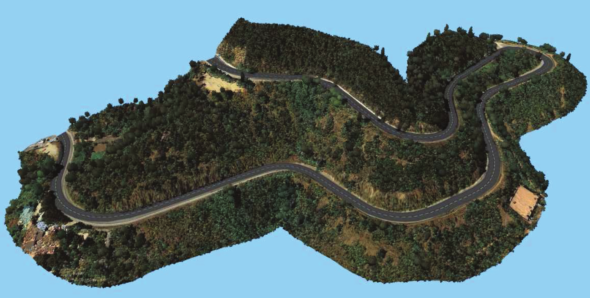
\includegraphics[width=\textwidth]{reconstructed_roadside_vegetation.png}
	\caption{Reconstructed roadside vegetation using orthophotos ~\cite{Andujar2014}}
\end{figure}

Explicit instancing methods provide extensive user control and freedom for the resulting virtual world. However, although some automation is provided, it is often limited. Therefore, albeit simplified, generating large virtual worlds can still be a lengthy process. \\

\subsection{Probabilistic Instancing} \label{Probabilistic Instancing}

Probabilistic instancing methods use statistical models in an attempt to produce adequate vegetation. These methods can be further split into two sub-categories which are discussed in further detail below: \textit{Radial distribution analysis} and \textit{Predefined ecotopes}.\\

\subsubsection{RADIAL DISTRIBUTION ANALYSIS}
Work by Emilien et al. \cite{Emilien}, Boudon et al. \cite{Boudon2007} and Lane et al. \cite{Lane2002} use radial distribution analysis to grasp the underlying layout of given input examplars. The data generated by the analysis stage can later be used to synthesise, at any scale, new point distributions which respect the characteristics of the input exemplar \cite{Oztireli2012}. \\
For example, by analysing the positions of individual plants in a small subset of a forest and using it as the input exemplar, it is possible to reproduce it at a much larger scale in order to model the full-size forest.\\

\paragraph{Analysis}
Generating the analytical data involves measuring the distances between individual points of different categories from the input examplar. For plant distribution analysis, the points represent individual plant instances and the categories represent the different species.\\

Before performing the analysis, the following parameters need to be configured:
\begin{itemize}
\item \textbf{R\textsubscript{min}}: The minimum distance from which point distances need to be analysed.\\
\item \textbf{R\textsubscript{max}}: The maximum distance after which point distances don't need to be analysed.\\
\item \textbf{Bin size}: When analysing the distances of given points, it is necessary to aggregate the points which reside at similar distances into bins. The bin size is the distance represented by a single bin.\\
\end{itemize}

A core part of radial distribution analysis is generating pair correlation histograms for each category pair combination. A pair correlation histogram \textit{H\textsubscript{AB}} represents the variation in the distance between points of of category \textit{C\textsubscript{A}} and \textit{C\textsubscript{B}} ranging from \textit{R\textsubscript{min}} to \textit{R\textsubscript{max}} in \textit{bin size} increments (figure \ref{Pair Correlation Histograms}) \\

\begin{figure}[h]
  \centering
	\label{Pair Correlation Histograms}
	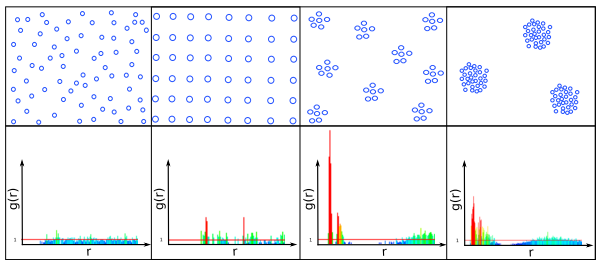
\includegraphics[width=\textwidth]{pair_correlation_histograms.png}
	\caption{Point distributions with associated pair correlation histogram \cite{Emilien2014}}
\end{figure}

To generate the pair correlation histogram \textit{H\textsubscript{AB}}, the algorithm iterates through each reference point of category \textit{C\textsubscript{A}} and for each destination point of category \textit{C\textsubscript{B}} at a distance between \textit{R\textsubscript{min}} and \textit{R\textsubscript{max}} increments the relevant bin in the histogram.\\
In figure \ref{Radial distribution analysis}, for example, are being measured the points that lie within the annular shell of radius \textit{r} with bin size \textit{d\textsubscript{r}} (area \textit{d\textsubscript{A}}). 

\begin{figure}[h]
  \centering
	\label{Radial distribution analysis}
	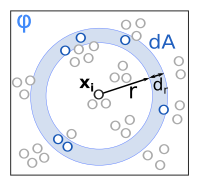
\includegraphics[natwidth=199,natheight=140]{radial_distribution_analysis.png}
	\caption{Radial distribution analysis]}
\end{figure}

The coverage area of annular shells are larger for bins being analysed at further distances. In other words, \textit{A\textsubscript{r}} < \textit{A\textsubscript{r+1}} where \textit{A\textsubscript{r}} is the area covered by the annular shell starting at distance \textit{r}. To counter for this, and the fact that there will naturally be more points in these larger annular shells, normalisation is performed. \\

The radial distribution analysis function \textit{h\textsubscript{rdf}} is as follows:\\
\begin{center}	
$h_{rdf}(k) = \sum_{x_{i} \in X} \sum_{y_{j} \in Y \&  
kd_{r} \leq d(x_{i}, y_{j}) < (k+1)d_{r} } \frac{A}{d_{A}n_{x}n_{y}} $
\end{center}
Where:
\begin{itemize}
\item \textit{hrdf(k)} is the k-th value of the pair wise histogram.
\item \textit{X} are the reference points.
\item \textit{Y} are the target points.
\item \textit{d\textsubscript{r}} is the annular shell width.
\item \textit{A} is the total analysed area.
\item \textit{n\textsubscript{x}} and \textit{n\textsubscript{y}} are the number of points of categories \textit{x} and \textit{y} respectively.
\item \textit{d\textsubscript{A}} is the area of the annular shell being analysed.
\end{itemize}

Conceptually, this formula calculates the variance from the average density of the target category at incremental distances from points of the reference category.

\paragraph{Reproduction}

In order to reproduce the distribution of the input exemplar, points must be added iteratively whilst matching as closely as possible the categorical point separation data calculated during the analysis stage. Arnaud et al. ~\cite{Emilien} use Metropolis-Hastings sampling ~\cite{Hurtut2009}. This technique involves performing a fixed number of birth-and-death perturbations. A change from the initial arrangement \textit{X} to the new arrangement \textit{X'} is accepted with probability \textit{R}, where:

\begin{center}
$ R = \frac{f(X')}{f(X}$
\end{center}
\textit{f(X)} is the probability density function (PDF) and is expressed as:\\

\begin{center}
$ f(X) = \prod_{C_{Y_{K}} \leq C_{X}} 
		 \prod_{x_{i} \in X}
		 \prod_{y_{i} \in Y_{k}} 
		 h_{X,Y_{k}}(d(x_{i},y_{j}))$
\end{center} 

Where:
\begin{itemize}
\item \textit{C\textsubscript{y}} and \textit{C\textsubscript{x}} represent categories \textit{Y} and \textit{X} respectively
\item \textit{X} are all points of category \textit{X}
\item \textit{Y} are all points of category \textit{Y}
\item h\textsubscript{X,Y\textsubscript{k}}(d(x\textsubscript{i}, y\textsubscript{j})) is the value retrieved from the pairwise histogram of categories \textit{X} and \textit{Y} given the distance between points \textit{x\textsubscript{i}} and \textit{y\textsubscript{i}}.
\end{itemize}
Intuitively, the PDF defines, given a set of points, the aggregate strength of the current distribution.\\

The main advantage of the probabilistic approach is computational efficiency. In the work by Arnaud et al. ~\cite{Emilien}, both analysis and reproduction is performed in near real-time. Another advantage is that specific specie properties are not needed. \\
The primary disadvantage of this approach is scalability. Given an input exemplar, the system will only be able to reproduce the given plant distribution characteristics. If a new plant is to be added to the forest, for example, a new input exemplar must be created. 

\subsubsection{Predefined ecotopes}
